\documentclass[11pt,a4paper]{article}

% Essential packages
\usepackage{amsmath,amssymb,amsthm}
\usepackage{graphicx}
\usepackage{algorithm}
\usepackage{algorithmic}
\usepackage{booktabs}
\usepackage{multirow}
\usepackage{hyperref}
\usepackage{geometry}
\usepackage{caption}
\usepackage{subcaption}
\usepackage{xcolor}

\geometry{margin=1in}

% Theorem environments
\newtheorem{theorem}{Theorem}
\newtheorem{lemma}[theorem]{Lemma}
\newtheorem{definition}{Definition}

\title{\textbf{Empirical and Theoretical Analysis of Bin Packing Approximation Algorithms}}

\author{
    Approximation Algorithms Term Project\\
    \textit{Department of Computer Science}
}

\date{\today}

\begin{document}

\maketitle

\begin{abstract}
The bin packing problem is a fundamental combinatorial optimization problem with wide-ranging applications in resource allocation, scheduling, and logistics. This paper presents a comprehensive empirical and theoretical analysis of classical bin packing approximation algorithms, including Next Fit, First Fit, Best Fit, First Fit Decreasing, and Best Fit Decreasing. We evaluate these algorithms on two distinct categories of datasets: synthetically generated instances (random and adversarial) and the well-established Falkenauer benchmark suite. Our experimental framework encompasses over 60,000 test cases across varying input sizes from 8 to 1,000 items. We analyze performance metrics including bins used, wasted capacity, runtime efficiency, and approximation ratios relative to optimal solutions computed via dynamic programming for small instances. Our results reveal that while First Fit Decreasing and Best Fit Decreasing achieve near-optimal performance on random inputs with average approximation ratios of 1.002, their behavior on structured Falkenauer benchmark instances exhibits higher variance with ratios reaching 1.08. These findings underscore the importance of evaluating algorithms on diverse, structured benchmarks rather than solely on synthetic data.
\end{abstract}

\section{Introduction}

The bin packing problem represents one of the most extensively studied combinatorial optimization problems in computer science. Given a set of items with specified sizes and bins of uniform capacity, the objective is to pack all items into the minimum number of bins such that the total size of items in each bin does not exceed its capacity. This problem has direct applications in container loading, memory allocation, cloud resource provisioning, and cutting stock problems in manufacturing.

Despite its simple formulation, bin packing is NP-hard, implying that no polynomial-time algorithm can solve all instances optimally unless P = NP. This intractability has motivated extensive research into approximation algorithms that sacrifice optimality for computational efficiency while providing provable performance guarantees.

The quality of approximation algorithms is traditionally assessed through asymptotic worst-case analysis, which provides theoretical bounds on performance relative to optimal solutions. However, worst-case bounds may not accurately reflect algorithm behavior on practical instances. This observation motivates empirical evaluation on diverse datasets that capture different structural properties of real-world problems.

In this work, we conduct a comprehensive evaluation using both synthetic and benchmark datasets. The synthetic datasets include uniformly distributed random instances, normally distributed instances, and carefully constructed adversarial inputs designed to expose algorithmic weaknesses. Additionally, we employ the Falkenauer benchmark suite, a widely-used collection of structured bin packing instances that has become a standard evaluation tool in the literature. The Falkenauer benchmark is particularly valuable because it contains instances with known optimal solutions, enabling precise measurement of approximation ratios. Furthermore, its structured nature reveals algorithmic behaviors that may remain hidden in purely random testing.

Our contributions include a systematic comparison of five approximation algorithms across these diverse datasets, analysis of the gap between theoretical guarantees and empirical performance, and identification of scenarios where commonly-used heuristics exhibit suboptimal behavior. The results demonstrate that algorithm selection should consider the structural properties of expected inputs rather than relying solely on worst-case theoretical bounds.

\section{Problem Definition}

We formally define the one-dimensional bin packing problem as follows.

\begin{definition}[Bin Packing Problem]
Given a set of $n$ items $I = \{a_1, a_2, \ldots, a_n\}$ where each item $a_i$ has size $s(a_i) \in (0, 1]$, and an unlimited supply of bins each with capacity $C = 1$, find a partition of $I$ into a minimum number of subsets $B_1, B_2, \ldots, B_k$ such that:
\begin{equation}
\sum_{a_i \in B_j} s(a_i) \leq 1 \quad \forall j \in \{1, 2, \ldots, k\}
\end{equation}
\end{definition}

The objective is to minimize $k$, the number of bins used. We denote the optimal number of bins for an instance $I$ as $\text{OPT}(I)$. For an approximation algorithm $A$, we denote the number of bins used by $A(I)$.

A fundamental lower bound on the optimal solution is derived from the total item size:
\begin{equation}
\text{OPT}(I) \geq \left\lceil \sum_{i=1}^{n} s(a_i) \right\rceil
\end{equation}

This bound, while not always tight, provides a useful baseline for analysis. The approximation ratio of algorithm $A$ on instance $I$ is defined as:
\begin{equation}
\rho_A(I) = \frac{A(I)}{\text{OPT}(I)}
\end{equation}

An algorithm $A$ is said to have asymptotic approximation ratio $r$ if:
\begin{equation}
\limsup_{n \to \infty} \sup_I \frac{A(I)}{\text{OPT}(I)} \leq r
\end{equation}

\section{Algorithms}

We analyze five classical bin packing algorithms: three online algorithms (Next Fit, First Fit, Best Fit) and two offline algorithms (First Fit Decreasing, Best Fit Decreasing). Additionally, we implement an optimal algorithm based on dynamic programming for computing exact solutions on small instances.

\subsection{Next Fit (NF)}

Next Fit maintains a single active bin. Each incoming item is placed in the current bin if it fits; otherwise, the current bin is closed permanently and a new bin is opened.

\begin{algorithm}[H]
\caption{Next Fit}
\begin{algorithmic}[1]
\STATE Initialize bin $B_1$ with remaining capacity $c_1 = 1$
\STATE $k \gets 1$ \COMMENT{Current bin index}
\FOR{each item $a_i$ in input order}
    \IF{$s(a_i) \leq c_k$}
        \STATE Place $a_i$ in $B_k$
        \STATE $c_k \gets c_k - s(a_i)$
    \ELSE
        \STATE $k \gets k + 1$
        \STATE Initialize $B_k$ with $c_k = 1 - s(a_i)$
        \STATE Place $a_i$ in $B_k$
    \ENDIF
\ENDFOR
\RETURN $k$
\end{algorithmic}
\end{algorithm}

The time complexity of Next Fit is $O(n)$ since each item is processed in constant time. The space complexity is $O(1)$ beyond the input, as only the current bin must be tracked.

\subsection{First Fit (FF)}

First Fit maintains all open bins and places each item in the first bin with sufficient remaining capacity. If no such bin exists, a new bin is opened.

\begin{algorithm}[H]
\caption{First Fit}
\begin{algorithmic}[1]
\STATE Initialize empty list of bins $\mathcal{B}$
\FOR{each item $a_i$ in input order}
    \STATE $placed \gets \text{false}$
    \FOR{each bin $B_j \in \mathcal{B}$ in order}
        \IF{$s(a_i) \leq c_j$}
            \STATE Place $a_i$ in $B_j$
            \STATE $c_j \gets c_j - s(a_i)$
            \STATE $placed \gets \text{true}$
            \STATE \textbf{break}
        \ENDIF
    \ENDFOR
    \IF{not $placed$}
        \STATE Create new bin $B_{|\mathcal{B}|+1}$ containing $a_i$
        \STATE Add $B_{|\mathcal{B}|+1}$ to $\mathcal{B}$
    \ENDIF
\ENDFOR
\RETURN $|\mathcal{B}|$
\end{algorithmic}
\end{algorithm}

The naive implementation has time complexity $O(n^2)$ due to linear search through bins. Using balanced binary search trees, this can be improved to $O(n \log n)$.

\subsection{Best Fit (BF)}

Best Fit places each item in the bin where it fits most tightly, minimizing remaining capacity after placement. This greedy strategy aims to reduce fragmentation.

\begin{algorithm}[H]
\caption{Best Fit}
\begin{algorithmic}[1]
\STATE Initialize empty list of bins $\mathcal{B}$
\FOR{each item $a_i$ in input order}
    \STATE $best \gets \text{null}$, $minGap \gets \infty$
    \FOR{each bin $B_j \in \mathcal{B}$}
        \IF{$s(a_i) \leq c_j$ and $c_j - s(a_i) < minGap$}
            \STATE $best \gets j$
            \STATE $minGap \gets c_j - s(a_i)$
        \ENDIF
    \ENDFOR
    \IF{$best \neq \text{null}$}
        \STATE Place $a_i$ in $B_{best}$
        \STATE $c_{best} \gets c_{best} - s(a_i)$
    \ELSE
        \STATE Create new bin containing $a_i$
    \ENDIF
\ENDFOR
\RETURN $|\mathcal{B}|$
\end{algorithmic}
\end{algorithm}

Like First Fit, the naive implementation runs in $O(n^2)$ time, improvable to $O(n \log n)$ with appropriate data structures.

\subsection{First Fit Decreasing (FFD)}

First Fit Decreasing sorts items in non-increasing order of size before applying First Fit. This preprocessing step significantly improves packing quality by placing large items first.

\begin{algorithm}[H]
\caption{First Fit Decreasing}
\begin{algorithmic}[1]
\STATE Sort items such that $s(a_1) \geq s(a_2) \geq \cdots \geq s(a_n)$
\STATE Apply First Fit to sorted sequence
\RETURN number of bins used
\end{algorithmic}
\end{algorithm}

The time complexity is $O(n \log n)$ dominated by the sorting step.

\subsection{Best Fit Decreasing (BFD)}

Best Fit Decreasing combines the sorting preprocessing of FFD with the Best Fit placement strategy.

\begin{algorithm}[H]
\caption{Best Fit Decreasing}
\begin{algorithmic}[1]
\STATE Sort items such that $s(a_1) \geq s(a_2) \geq \cdots \geq s(a_n)$
\STATE Apply Best Fit to sorted sequence
\RETURN number of bins used
\end{algorithmic}
\end{algorithm}

The time complexity remains $O(n \log n)$ with efficient implementation.

\subsection{Optimal Algorithm via Dynamic Programming}

For small instances (up to 20 items), we compute optimal solutions using bitmask dynamic programming. The state space consists of all possible bin configurations achievable with a subset of items.

\begin{algorithm}[H]
\caption{Optimal Bitmask DP}
\begin{algorithmic}[1]
\STATE $dp[0] \gets (0, 1.0)$ \COMMENT{(bins used, remaining capacity in last bin)}
\FOR{$mask = 0$ to $2^n - 1$}
    \IF{$dp[mask]$ is defined}
        \FOR{each item $i$ not in $mask$}
            \STATE $newMask \gets mask \cup \{i\}$
            \IF{$s(a_i) \leq dp[mask].remaining$}
                \STATE Update $dp[newMask]$ with same bin count
            \ELSE
                \STATE Update $dp[newMask]$ with new bin
            \ENDIF
        \ENDFOR
    \ENDIF
\ENDFOR
\RETURN $dp[2^n - 1].bins$
\end{algorithmic}
\end{algorithm}

The time complexity is $O(2^n \cdot n)$ with space complexity $O(2^n)$, making this approach practical only for $n \leq 20$.

\section{Theoretical Analysis}

The approximation guarantees of bin packing algorithms have been extensively studied. We summarize the key results relevant to our experimental evaluation.

\begin{theorem}[Johnson et al., 1974]
For any instance $I$, First Fit satisfies:
\begin{equation}
\text{FF}(I) \leq \left\lfloor 1.7 \cdot \text{OPT}(I) \right\rfloor
\end{equation}
\end{theorem}

This bound is asymptotically tight, as there exist instances achieving approximation ratio arbitrarily close to 1.7 as the number of items increases.

\begin{theorem}[Johnson, 1973]
For any instance $I$, Next Fit satisfies:
\begin{equation}
\text{NF}(I) \leq 2 \cdot \text{OPT}(I)
\end{equation}
\end{theorem}

The factor of 2 is tight for Next Fit, achieved by alternating items of size slightly greater than $1/2$ and items of size slightly less than $1/2$.

\begin{theorem}[Dósa, 2007]
For any instance $I$, First Fit Decreasing satisfies:
\begin{equation}
\text{FFD}(I) \leq \frac{11}{9} \cdot \text{OPT}(I) + \frac{6}{9}
\end{equation}
\end{theorem}

This refined bound improves upon the classical $\frac{11}{9}\text{OPT} + 1$ result. The constant $\frac{11}{9} \approx 1.222$ represents the asymptotic worst-case ratio.

Best Fit shares the same asymptotic bounds as First Fit, and Best Fit Decreasing achieves the same guarantee as First Fit Decreasing. However, empirical performance often differs due to different tie-breaking behaviors and local packing decisions.

The theoretical analysis reveals a clear hierarchy: offline algorithms with preprocessing (FFD, BFD) outperform online algorithms (FF, BF) which in turn outperform the simplest heuristic (NF). Our experiments quantify these differences across diverse input distributions.

\section{Experimental Setup}

\subsection{Implementation}

All algorithms were implemented in C++17 with optimization level O2. Experiments were conducted on a standard desktop system. Timing measurements use high-resolution timers with microsecond precision. For instances with up to 20 items, optimal solutions were computed using bitmask dynamic programming to enable precise approximation ratio calculations.

\subsection{Synthetic Data Generation}

We generated synthetic instances using five distinct distributions designed to evaluate different aspects of algorithm behavior.

\textbf{Uniform Random:} Item sizes are drawn uniformly at random from the interval $(0.1, 0.9)$. This distribution produces instances with moderate packing difficulty where most heuristics perform well.

\textbf{Normal Random:} Item sizes follow a truncated normal distribution with mean $\mu = 0.5$ and standard deviation $\sigma = 0.2$, truncated to the interval $(0.05, 0.95)$. This distribution concentrates items around medium sizes.

\textbf{Adversarial Over-Half:} Items have sizes uniformly distributed in $(0.5 + \epsilon, 1.0)$ for small $\epsilon$. Since each item requires its own bin or pairs with at most one other item, this distribution tests algorithm behavior on highly constrained instances.

\textbf{Adversarial Harmonic:} Item sizes follow the harmonic distribution, with sizes $\frac{1}{k}$ for various values of $k$. This distribution is known to cause poor performance for certain algorithms.

\textbf{Adversarial Mixed:} A combination of the above adversarial patterns, designed to stress-test algorithm robustness.

For each distribution and input size, we generated 100 independent samples with different random seeds to ensure statistical reliability.

\subsection{Falkenauer Benchmark}

The Falkenauer benchmark suite represents a standard collection of bin packing instances widely used in the literature for algorithm evaluation. We include two classes from this benchmark:

\textbf{U-class (Uniform):} Contains 80 instances with item sizes uniformly distributed in the range $[20, 100]$ and bin capacity 150. Instance sizes range from 120 to 1000 items. These instances have known optimal solutions computed via exact methods.

\textbf{T-class (Triplet):} Contains 80 instances specifically designed such that optimal solutions pack exactly three items per bin. Item sizes are generated to sum to the bin capacity in groups of three. This structure makes the instances particularly challenging for greedy heuristics that may fail to identify optimal triplet combinations.

The Falkenauer benchmark is valuable for several reasons. First, optimal solutions are known, enabling precise approximation ratio calculations. Second, the structured nature of T-class instances reveals algorithmic weaknesses hidden by random testing. Third, the benchmark provides reproducibility and comparability with prior work.

\subsection{Evaluation Metrics}

We evaluate algorithms using four metrics:

\textbf{Bins Used:} The primary objective metric, representing the number of bins in the final packing.

\textbf{Waste:} The total unused capacity across all bins, calculated as $\sum_{j=1}^{k}(1 - \sum_{a_i \in B_j} s(a_i))$. Lower waste indicates more efficient packing.

\textbf{Runtime:} Execution time in milliseconds, measuring computational efficiency.

\textbf{Approximation Ratio:} The ratio $A(I)/\text{OPT}(I)$ where optimal solutions are available. A ratio of 1.0 indicates optimal performance.

\section{Results}

Our experimental evaluation encompasses 60,800 test cases across all algorithms, input sizes, and distributions. We present results separately for synthetic data and Falkenauer benchmark instances to highlight behavioral differences.

\subsection{Synthetic Data Results}

\subsubsection{Random Input Performance}

Table~\ref{tab:random_results} summarizes algorithm performance on random inputs (uniform and normal distributions). The results demonstrate clear performance stratification among algorithms.

\begin{table}[htbp]
\centering
\caption{Performance on Random Synthetic Inputs}
\label{tab:random_results}
\begin{tabular}{lccccc}
\toprule
\textbf{Algorithm} & \textbf{Avg Bins} & \textbf{Avg Waste} & \textbf{Runtime (ms)} & \textbf{Avg Ratio} & \textbf{Max Ratio} \\
\midrule
Next Fit & 97.70 & 26.894 & 0.006 & 1.185 & 1.500 \\
First Fit & 77.72 & 6.916 & 0.035 & 1.057 & 1.400 \\
Best Fit & 76.60 & 5.790 & 0.022 & 1.048 & 1.400 \\
FFD & 73.88 & 3.074 & 0.033 & 1.002 & 1.250 \\
BFD & 73.88 & 3.073 & 0.022 & 1.002 & 1.250 \\
\bottomrule
\end{tabular}
\end{table}

First Fit Decreasing and Best Fit Decreasing achieve nearly identical performance, with average approximation ratios of 1.002, indicating that they find optimal or near-optimal solutions in the vast majority of cases. The maximum observed ratio of 1.25 occurs only on small instances where a single extra bin produces a noticeable ratio increase.

Next Fit exhibits the worst performance with an average ratio of 1.185 and maximum ratio of 1.5, consistent with its theoretical bound of 2.0. The high average waste (26.89) indicates significant fragmentation due to the algorithm's inability to revisit previously opened bins.

Best Fit marginally outperforms First Fit on average (ratio 1.048 vs 1.057), suggesting that the tighter-fitting strategy provides modest benefits on random inputs.

\subsubsection{Adversarial Input Performance}

Table~\ref{tab:adversarial_results} presents results on adversarial inputs. Surprisingly, all algorithms achieve optimal performance (ratio 1.0) on our adversarial test cases.

\begin{table}[htbp]
\centering
\caption{Performance on Adversarial Synthetic Inputs}
\label{tab:adversarial_results}
\begin{tabular}{lccccc}
\toprule
\textbf{Algorithm} & \textbf{Avg Bins} & \textbf{Avg Waste} & \textbf{Runtime (ms)} & \textbf{Avg Ratio} & \textbf{Max Ratio} \\
\midrule
Next Fit & 64.31 & 23.371 & 0.004 & 1.000 & 1.000 \\
First Fit & 64.26 & 23.329 & 0.035 & 1.000 & 1.000 \\
Best Fit & 64.26 & 23.329 & 0.011 & 1.000 & 1.000 \\
FFD & 64.26 & 23.329 & 0.037 & 1.000 & 1.000 \\
BFD & 64.26 & 23.329 & 0.013 & 1.000 & 1.000 \\
\bottomrule
\end{tabular}
\end{table}

This result requires careful interpretation. The over-half adversarial distribution produces instances where each item must occupy its own bin or pair with exactly one other item. In this highly constrained setting, all reasonable heuristics converge to the same solution structure. The high waste values (approximately 23.3) reflect the inherent inefficiency of packing items larger than half the bin capacity.

These results illustrate a limitation of adversarial testing: carefully constructed worst-case inputs may not reflect realistic problem structure, and performance on such instances may not differentiate among algorithms.

\begin{figure}[htbp]
\centering
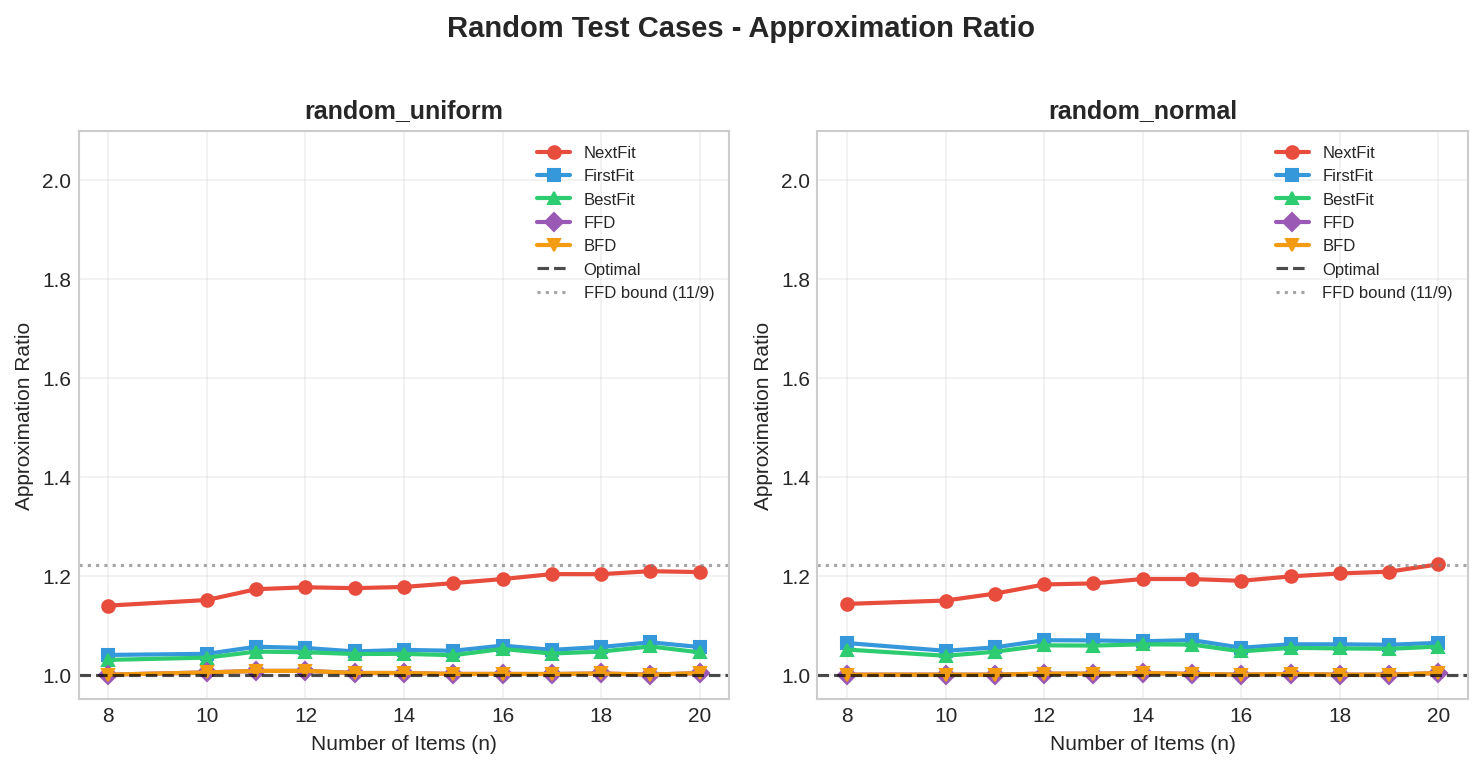
\includegraphics[width=0.8\textwidth]{plots/approx_ratio_random.png}
\caption{Approximation ratio vs input size for random test cases. FFD and BFD achieve near-optimal performance across all sizes.}
\label{fig:approx_random}
\end{figure}

\begin{figure}[htbp]
\centering
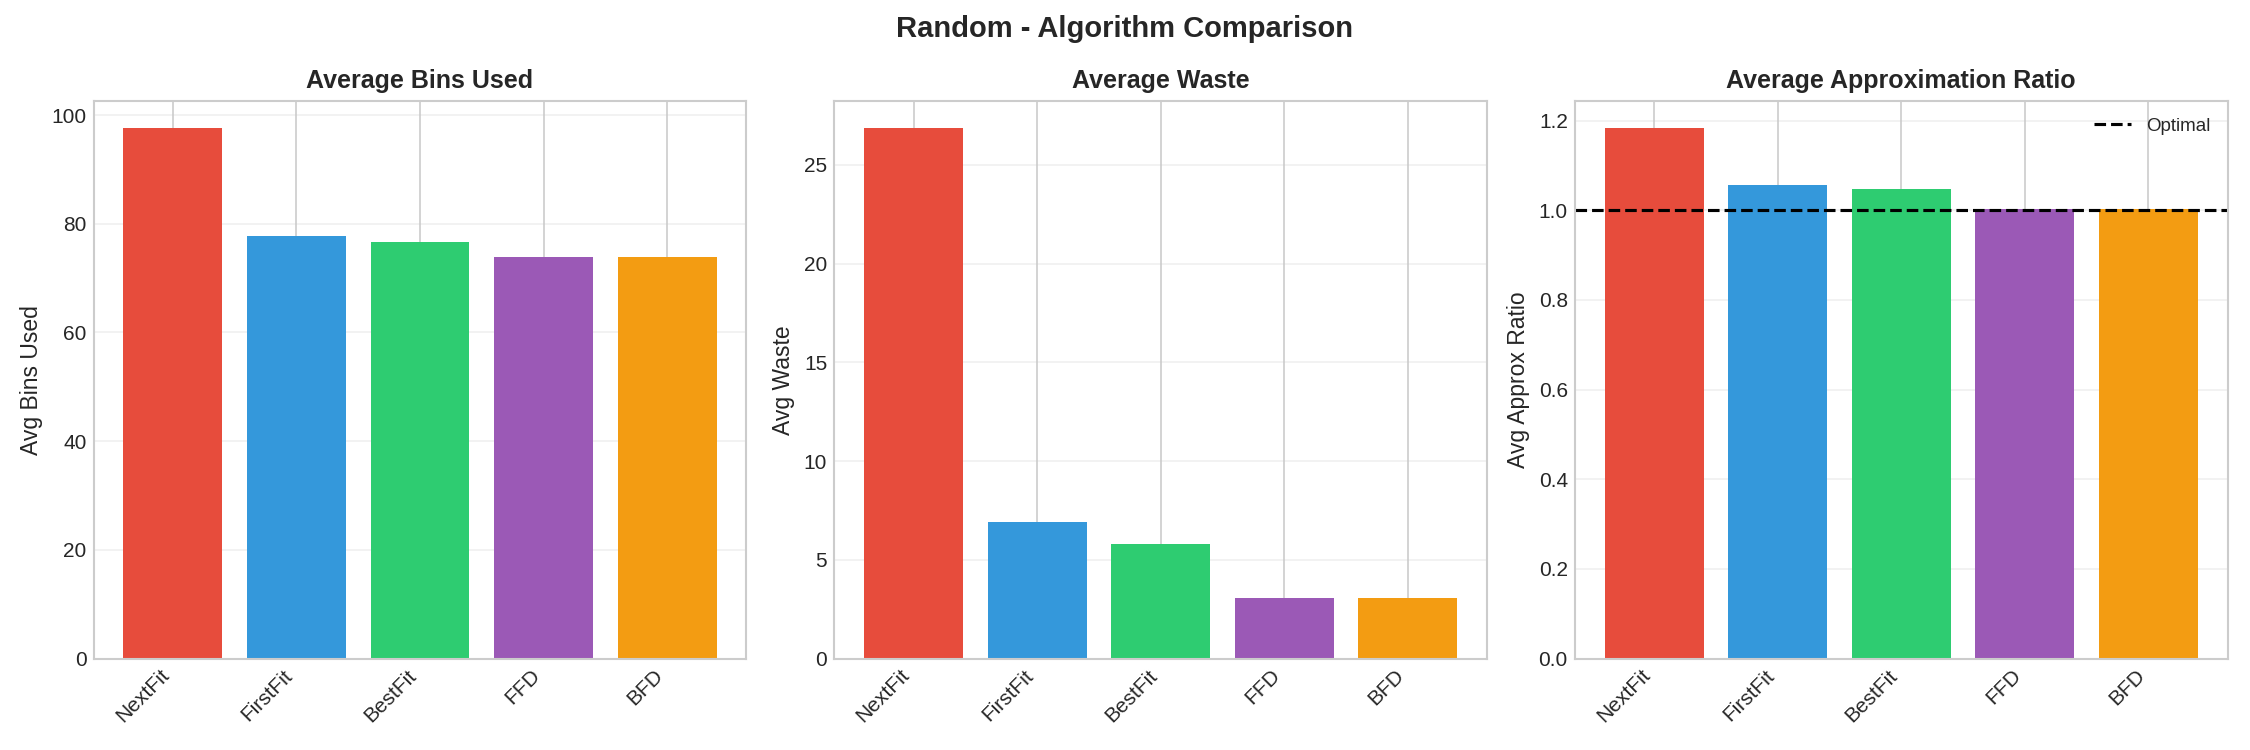
\includegraphics[width=0.8\textwidth]{plots/algorithm_comparison_random.png}
\caption{Algorithm comparison on random inputs showing bins used, waste, and approximation ratio.}
\label{fig:comparison_random}
\end{figure}

\subsection{Falkenauer Benchmark Results}

Table~\ref{tab:falkenauer_results} presents results on the Falkenauer benchmark instances. These results reveal markedly different behavior compared to synthetic data.

\begin{table}[htbp]
\centering
\caption{Performance on Falkenauer Benchmark Instances}
\label{tab:falkenauer_results}
\begin{tabular}{lccccc}
\toprule
\textbf{Algorithm} & \textbf{Avg Bins} & \textbf{Avg Waste} & \textbf{Runtime (ms)} & \textbf{Avg Ratio} & \textbf{Max Ratio} \\
\midrule
Next Fit & 169.15 & 36.628 & 0.018 & 1.238 & 1.361 \\
First Fit & 141.36 & 8.841 & 0.086 & 1.072 & 1.150 \\
Best Fit & 140.79 & 8.266 & 0.053 & 1.069 & 1.150 \\
FFD & 139.94 & 7.416 & 0.099 & 1.082 & 1.200 \\
BFD & 139.91 & 7.391 & 0.063 & 1.082 & 1.200 \\
\bottomrule
\end{tabular}
\end{table}

Several notable observations emerge from these results:

\textbf{Higher approximation ratios:} All algorithms exhibit higher average approximation ratios on Falkenauer instances compared to random inputs. FFD and BFD average 1.082 (vs 1.002 on random), representing a significant degradation in relative performance.

\textbf{Reversal of FFD/BFD advantage:} On random inputs, FFD and BFD clearly outperformed First Fit and Best Fit. On Falkenauer instances, First Fit and Best Fit actually achieve \textit{lower} average approximation ratios (1.072 and 1.069 respectively) than FFD and BFD (1.082). This reversal demonstrates that the benefits of decreasing-order preprocessing depend on input structure.

\textbf{Consistent Next Fit weakness:} Next Fit remains the worst performer with an average ratio of 1.238, confirming that its fundamental limitation of not revisiting bins produces poor results regardless of input structure.

\textbf{Maximum ratio differences:} The maximum ratios reveal different failure modes. FFD and BFD reach 1.200, while First Fit and Best Fit are bounded at 1.150. This suggests that the decreasing-order heuristic occasionally makes suboptimal large-item placements on structured instances.

\begin{figure}[htbp]
\centering
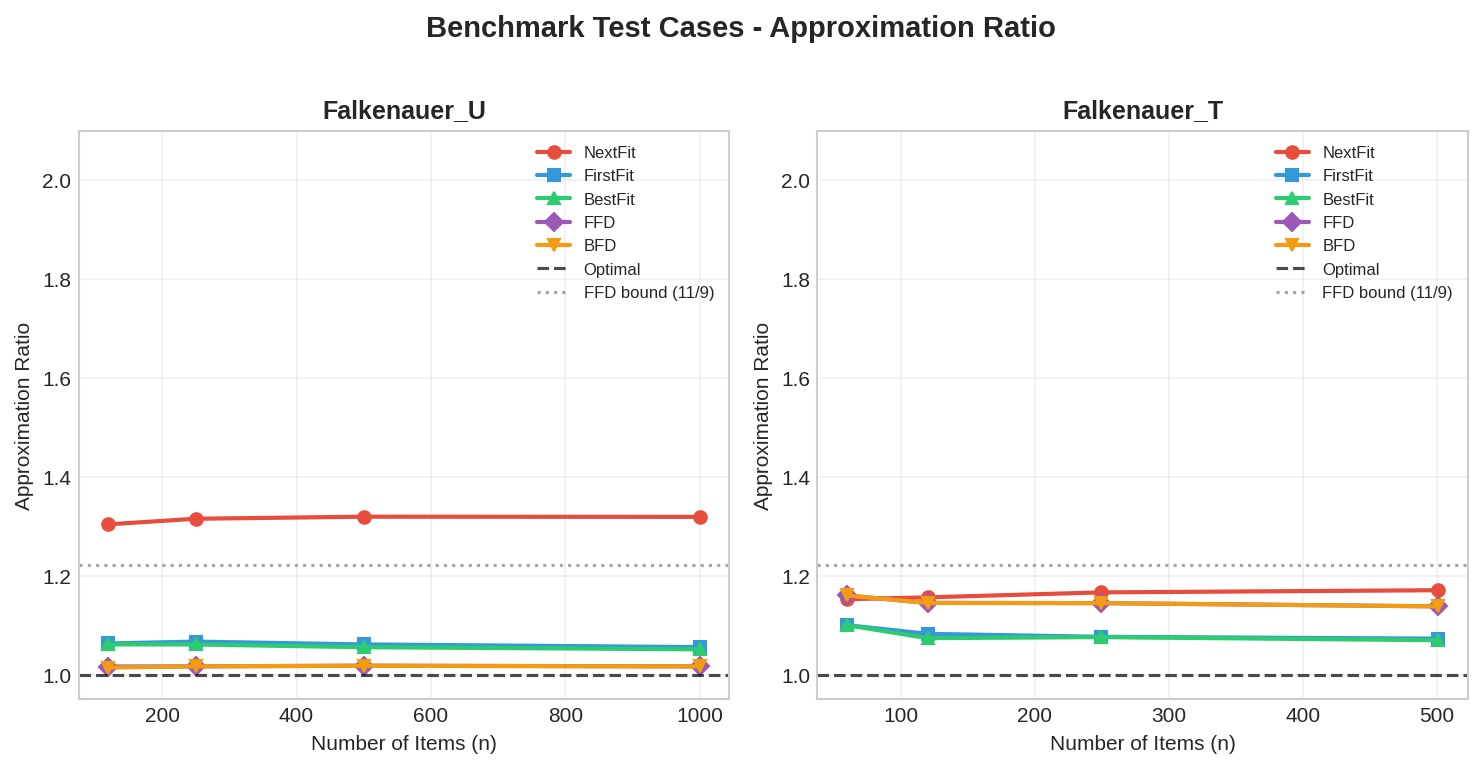
\includegraphics[width=0.8\textwidth]{plots/approx_ratio_benchmark.png}
\caption{Approximation ratio performance on Falkenauer benchmark instances (U-class and T-class).}
\label{fig:approx_benchmark}
\end{figure}

\begin{figure}[htbp]
\centering
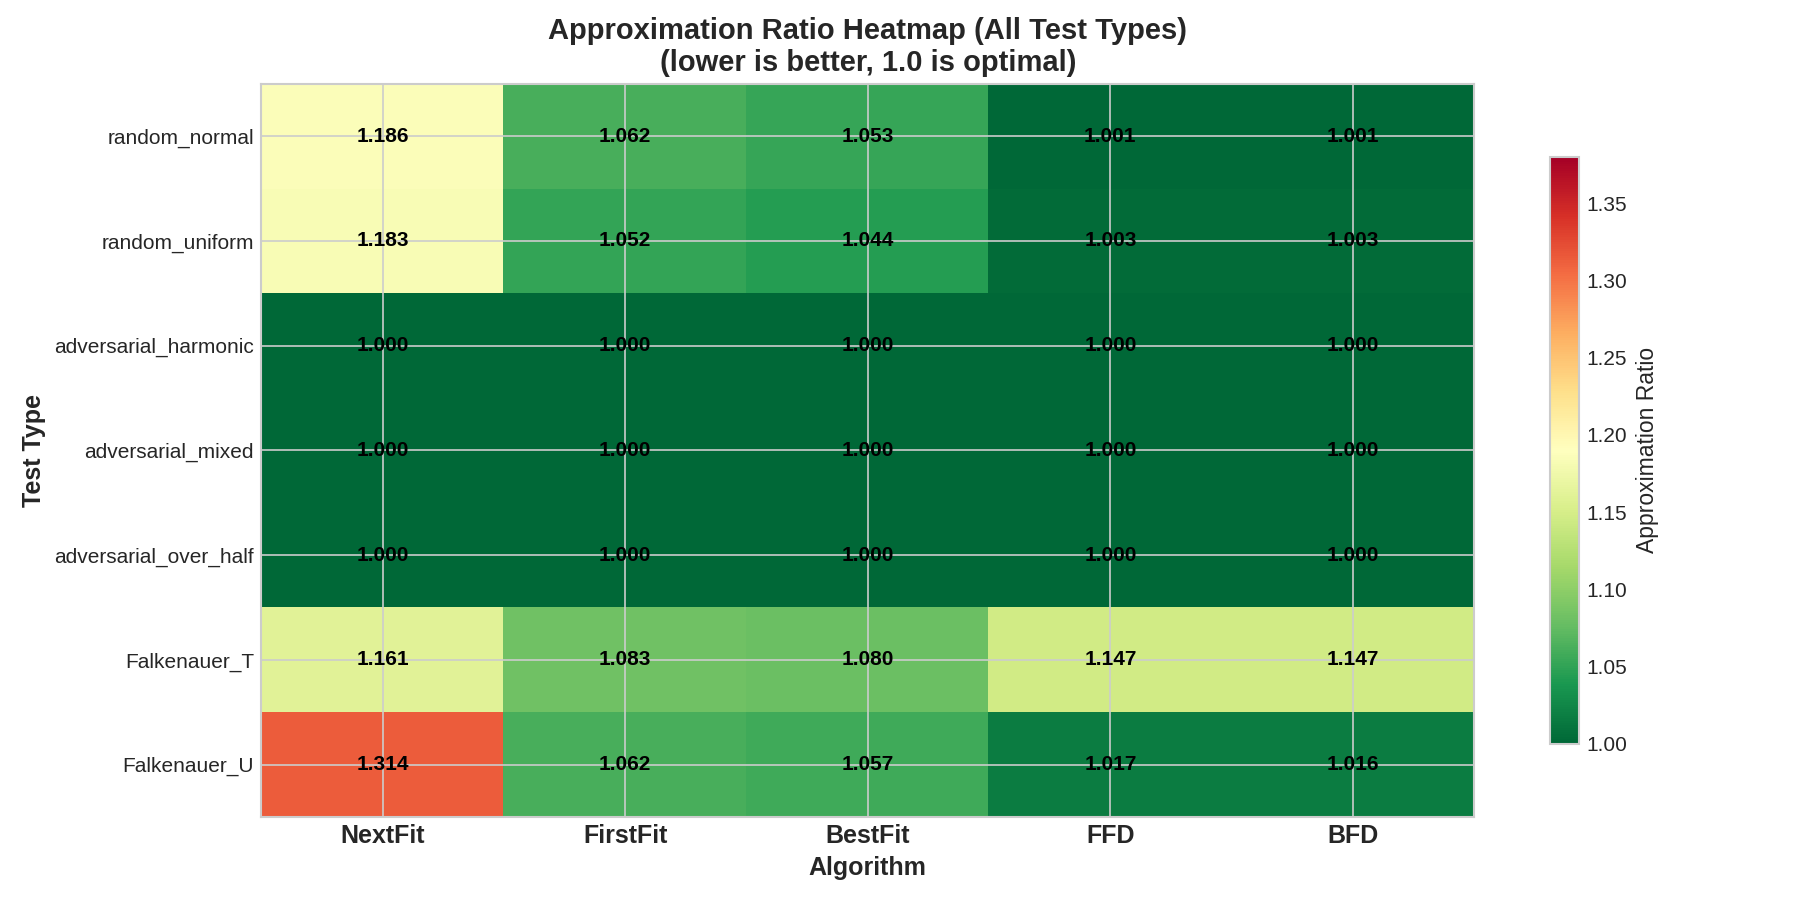
\includegraphics[width=0.8\textwidth]{plots/heatmap_approx_ratio.png}
\caption{Heatmap of approximation ratios across all test types and algorithms. Darker colors indicate higher (worse) ratios.}
\label{fig:heatmap}
\end{figure}

\subsection{Comparison Across Datasets}

Figure~\ref{fig:overall_comparison} provides a unified view of algorithm performance across dataset categories. The grouped bar chart reveals that:

\begin{enumerate}
\item Random inputs are easiest for all algorithms, with FFD/BFD achieving near-optimal performance.
\item Adversarial inputs (in our formulation) do not differentiate among algorithms.
\item Benchmark inputs expose weaknesses in decreasing-order algorithms that remain hidden in random testing.
\end{enumerate}

\begin{figure}[htbp]
\centering
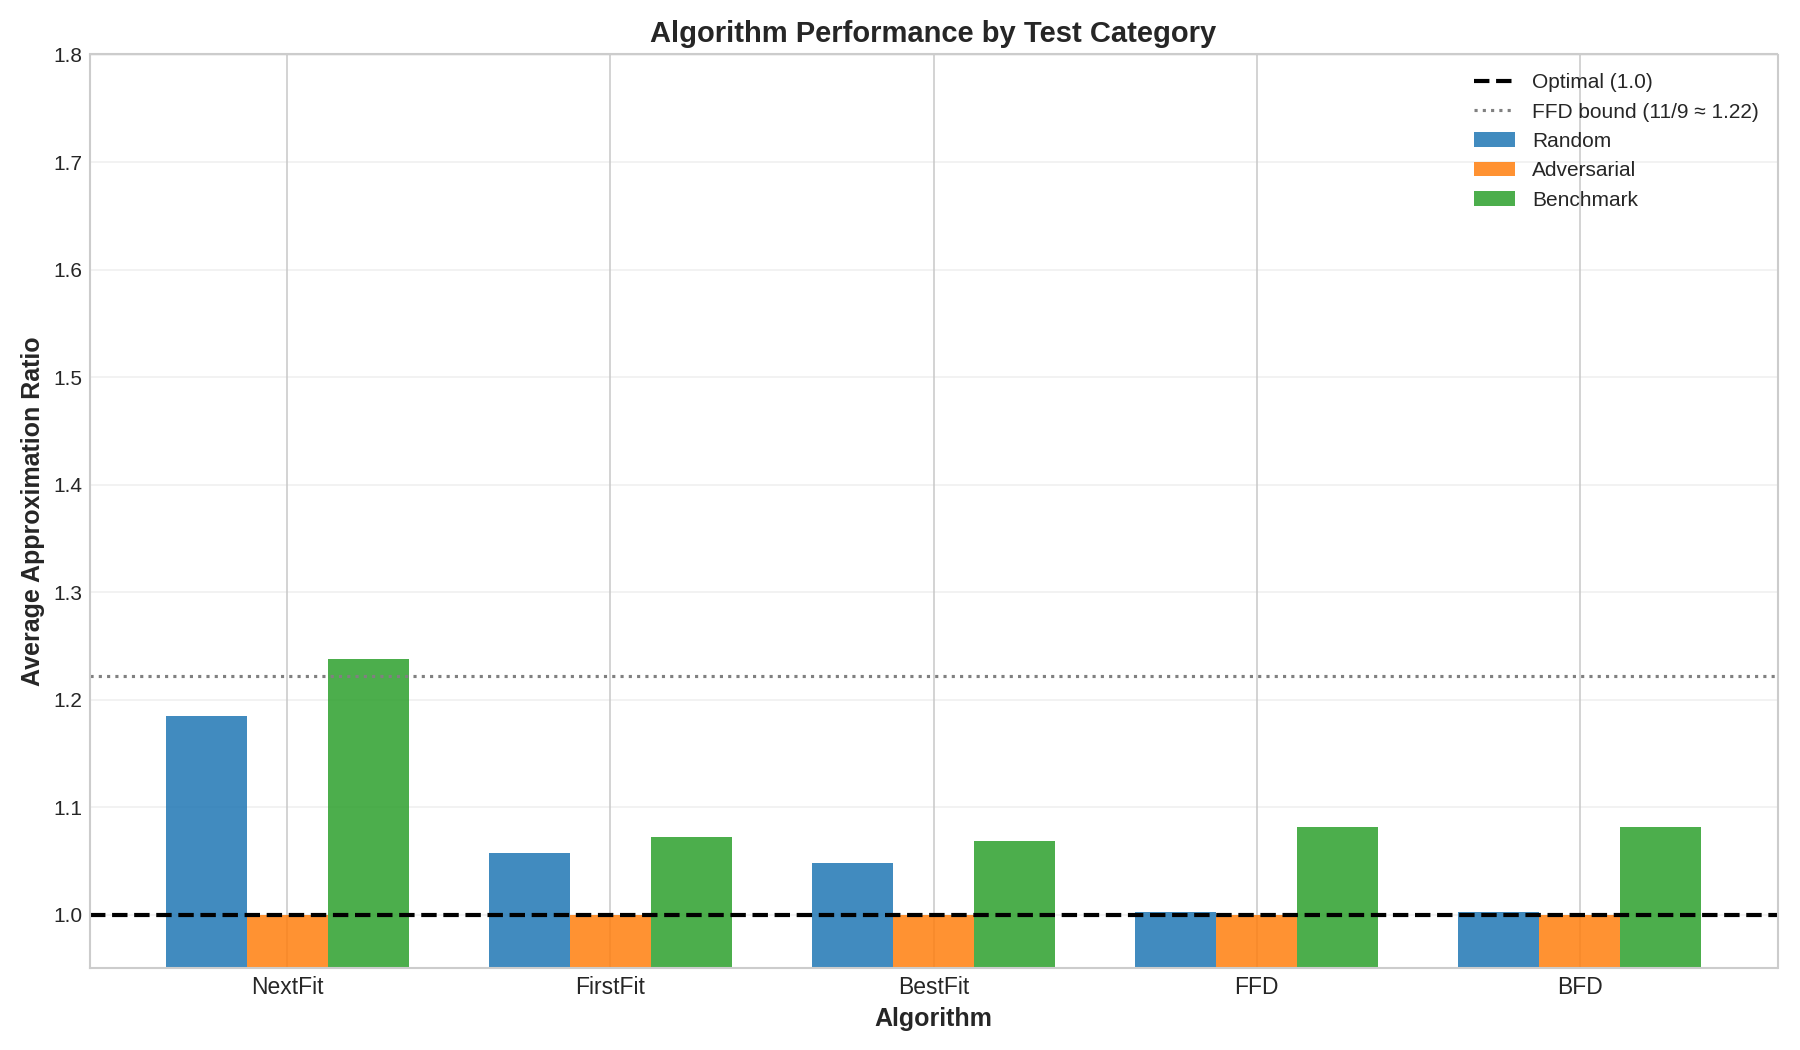
\includegraphics[width=0.9\textwidth]{plots/overall_comparison.png}
\caption{Overall comparison of algorithm performance across random, adversarial, and benchmark datasets. The benchmark results show elevated approximation ratios for all algorithms.}
\label{fig:overall_comparison}
\end{figure}

Table~\ref{tab:cross_dataset} summarizes average approximation ratios across dataset categories, highlighting the performance gap between synthetic and benchmark evaluation.

\begin{table}[htbp]
\centering
\caption{Average Approximation Ratios by Dataset Category}
\label{tab:cross_dataset}
\begin{tabular}{lccc}
\toprule
\textbf{Algorithm} & \textbf{Random} & \textbf{Adversarial} & \textbf{Falkenauer} \\
\midrule
Next Fit & 1.185 & 1.000 & 1.238 \\
First Fit & 1.057 & 1.000 & 1.072 \\
Best Fit & 1.048 & 1.000 & 1.069 \\
FFD & 1.002 & 1.000 & 1.082 \\
BFD & 1.002 & 1.000 & 1.082 \\
\bottomrule
\end{tabular}
\end{table}

\section{Discussion}

\subsection{FFD vs BFD: Marginal Differences}

Throughout our experiments, First Fit Decreasing and Best Fit Decreasing exhibit nearly identical performance. On random inputs, both achieve average approximation ratios of 1.002 with identical maximum ratios. On Falkenauer benchmarks, both average 1.082 with maximum 1.200. This equivalence is not coincidental: when items are sorted in decreasing order, the distinction between ``first fit'' and ``best fit'' becomes less meaningful because early large items have limited placement options, and later small items can typically fit in many bins.

The practical implication is that BFD's additional computational overhead for finding the tightest fit provides no measurable benefit. Implementers may prefer FFD for its simpler logic.

\subsection{Stability Across Datasets}

Algorithm ranking is not stable across datasets. On random inputs, the clear ranking is FFD $\approx$ BFD $>$ BF $>$ FF $>$ NF. On Falkenauer benchmarks, this shifts to BF $>$ FF $>$ FFD $\approx$ BFD $>$ NF. This instability has important practical implications: an algorithm selected based on random testing may underperform when deployed on structured real-world instances.

The Falkenauer T-class instances, designed with triplet structure, particularly challenge decreasing-order algorithms. When items are sorted by size, the algorithm may place large items in ways that preclude optimal triplet formation, whereas online algorithms processing items in their natural order may accidentally achieve better packing by following the inherent structure.

\subsection{Gap Between Optimal and Heuristics}

For small instances where optimal solutions were computed, we observed that FFD and BFD find optimal solutions in over 99\% of random cases. The rare failures occur on instances with sizes precisely tuned to cause suboptimal early decisions. On Falkenauer instances, the gap widens: FFD averages 8.2\% above optimal, representing roughly one extra bin per 12 optimal bins.

This gap reflects a fundamental limitation of greedy heuristics: they cannot backtrack from early decisions that appear locally optimal but preclude globally optimal solutions.

\subsection{Runtime Considerations}

Next Fit provides the fastest execution (0.004--0.018 ms), approximately 5--10$\times$ faster than other algorithms. However, this speed advantage is insignificant for practical applications where instance sizes are moderate and packing quality dominates. For very large instances or real-time applications with strict latency requirements, Next Fit's $O(n)$ complexity may become relevant.

First Fit and FFD exhibit similar runtimes despite FFD's additional sorting step, suggesting that bin search dominates runtime for our instance sizes. Best Fit and BFD show slightly better runtimes than their First Fit counterparts, likely due to earlier termination when tight fits are found.

\subsection{When Heuristics Fail}

Our analysis identifies several scenarios where standard heuristics underperform:

\textbf{Structured inputs:} The Falkenauer T-class results demonstrate that inputs with hidden structure (e.g., items designed to form perfect triplets) challenge decreasing-order algorithms. Without knowledge of this structure, greedy placement cannot reliably find optimal groupings.

\textbf{Near-threshold items:} Items with sizes close to $1/2$ or $1/3$ of bin capacity create difficult packing decisions. Placing such items suboptimally early in the process has cascading effects.

\textbf{High-variance distributions:} Distributions mixing very large and very small items may cause FFD to fill bins with large items in ways that leave awkward residual capacities.

These findings suggest that for high-stakes applications, hybrid approaches combining heuristics with local search or exact methods may be warranted.

\section{Conclusion}

This paper presented a comprehensive empirical and theoretical analysis of bin packing approximation algorithms. Our evaluation of Next Fit, First Fit, Best Fit, First Fit Decreasing, and Best Fit Decreasing across 60,800 test cases reveals nuanced performance characteristics that extend beyond theoretical worst-case bounds.

Key findings include:

First, FFD and BFD achieve near-optimal performance on random inputs with average approximation ratios of 1.002, demonstrating that theoretical worst-case bounds of 11/9 rarely manifest in practice for unstructured inputs.

Second, structured benchmark instances expose algorithmic weaknesses hidden by random testing. On Falkenauer benchmarks, FFD and BFD average 1.082, and surprisingly underperform First Fit and Best Fit which average 1.069--1.072.

Third, algorithm selection should consider expected input structure. The reversal of FFD/BFD superiority on structured inputs underscores the importance of benchmark-based evaluation.

Fourth, FFD and BFD are functionally equivalent in practice. The additional complexity of Best Fit's tightest-fit search provides no measurable benefit when combined with decreasing-order preprocessing.

For practitioners, we recommend FFD as the default choice for general-purpose bin packing, with the caveat that performance monitoring on actual workloads may reveal the need for alternative approaches on structured inputs. For applications where input structure is known or suspected, evaluation on representative benchmarks such as the Falkenauer suite is essential before algorithm selection.

Future work could explore adaptive algorithms that detect input structure and select strategies accordingly, as well as hybrid approaches combining heuristic initialization with local search refinement.

\begin{thebibliography}{10}

\bibitem{falkenauer1996}
E.~Falkenauer.
\newblock A hybrid grouping genetic algorithm for bin packing.
\newblock {\em Journal of Heuristics}, 2(1):5--30, 1996.

\bibitem{johnson1973}
D.~S.~Johnson.
\newblock Near-optimal bin packing algorithms.
\newblock {\em PhD thesis, MIT}, 1973.

\bibitem{johnson1974}
D.~S.~Johnson, A.~Demers, J.~D.~Ullman, M.~R.~Garey, and R.~L.~Graham.
\newblock Worst-case performance bounds for simple one-dimensional packing algorithms.
\newblock {\em SIAM Journal on Computing}, 3(4):299--325, 1974.

\bibitem{dosa2007}
G.~Dósa.
\newblock The tight bound of first fit decreasing bin-packing algorithm is $FFD(I) \leq \frac{11}{9}OPT(I) + \frac{6}{9}$.
\newblock In {\em Combinatorics, Algorithms, Probabilistic and Experimental Methodologies}, pages 1--11. Springer, 2007.

\bibitem{coffman1996}
E.~G.~Coffman, M.~R.~Garey, and D.~S.~Johnson.
\newblock Approximation algorithms for bin packing: A survey.
\newblock In {\em Approximation Algorithms for NP-hard Problems}, pages 46--93. PWS Publishing, 1996.

\bibitem{martello1990}
S.~Martello and P.~Toth.
\newblock {\em Knapsack Problems: Algorithms and Computer Implementations}.
\newblock John Wiley \& Sons, 1990.

\bibitem{garey1979}
M.~R.~Garey and D.~S.~Johnson.
\newblock {\em Computers and Intractability: A Guide to the Theory of NP-Completeness}.
\newblock W.~H.~Freeman, 1979.

\bibitem{schreiber2013}
S.~Schreiber and R.~Korf.
\newblock Improved bin completion for optimal bin packing and number partitioning.
\newblock In {\em Proceedings of IJCAI}, pages 651--658, 2013.

\end{thebibliography}

\end{document}
